% Chapter 1: Introduction to Time Series Analysis
% Harvard-quality academic presentation
% Bachelor program, Bucharest University of Economic Studies

\documentclass[9pt, aspectratio=169, t]{beamer}

% Ensure content fits on slides
\setbeamersize{text margin left=8mm, text margin right=8mm}

% Suppress tiny overfull warnings (under 2pt)
\hfuzz=2pt

%=============================================================================
% THEME AND STYLE CONFIGURATION
%=============================================================================
\usetheme{default}
% Using default theme for clean header/footer control

% Color Palette (matching Redispatch PDF)
\definecolor{MainBlue}{RGB}{26, 58, 110}
\definecolor{AccentBlue}{RGB}{26, 58, 110}
\definecolor{IDAred}{RGB}{205, 0, 0}
\definecolor{DarkGray}{RGB}{51, 51, 51}
\definecolor{MediumGray}{RGB}{128, 128, 128}
\definecolor{LightGray}{RGB}{248, 248, 248}
\definecolor{VeryLightGray}{RGB}{235, 235, 235}
\definecolor{KeynoteGray}{RGB}{218, 218, 218}
\definecolor{SectionGray}{RGB}{120, 120, 120}
\definecolor{FooterGray}{RGB}{100, 100, 100}
\definecolor{Crimson}{RGB}{220, 53, 69}
\definecolor{Forest}{RGB}{46, 125, 50}
\definecolor{Amber}{RGB}{181, 133, 63}
\definecolor{Orange}{RGB}{230, 126, 34}
\definecolor{Purple}{RGB}{142, 68, 173}

% Gradient background (exact Keynote 315° gradient: white to RGB 218,218,218)
\setbeamertemplate{background}{%
    \begin{tikzpicture}[remember picture, overlay]
        \shade[shading=axis, shading angle=315,
        top color=white, bottom color=KeynoteGray]
        (current page.south west) rectangle (current page.north east);
    \end{tikzpicture}%
}
% Fallback solid color for compatibility
\setbeamercolor{background canvas}{bg=}

\setbeamercolor{palette primary}{bg=MainBlue, fg=white}
\setbeamercolor{palette secondary}{bg=MainBlue!85, fg=white}
\setbeamercolor{palette tertiary}{bg=MainBlue!70, fg=white}
\setbeamercolor{structure}{fg=MainBlue}
\setbeamercolor{title}{fg=IDAred}
\setbeamercolor{frametitle}{fg=IDAred, bg=}
\setbeamercolor{block title}{bg=MainBlue, fg=white}
\setbeamercolor{block body}{bg=VeryLightGray, fg=DarkGray}
\setbeamercolor{block title alerted}{bg=Crimson, fg=white}
\setbeamercolor{block body alerted}{bg=Crimson!8, fg=DarkGray}
\setbeamercolor{block title example}{bg=Forest, fg=white}
\setbeamercolor{block body example}{bg=Forest!8, fg=DarkGray}
\setbeamercolor{item}{fg=MainBlue}

% Footer colors (override Madrid theme blue)
\setbeamercolor{author in head/foot}{fg=FooterGray, bg=}
\setbeamercolor{title in head/foot}{fg=FooterGray, bg=}
\setbeamercolor{date in head/foot}{fg=FooterGray, bg=}
\setbeamercolor{section in head/foot}{fg=FooterGray, bg=}
\setbeamercolor{subsection in head/foot}{fg=FooterGray, bg=}

% Bullet styles (apply everywhere including blocks)
\setbeamertemplate{itemize item}{\color{MainBlue}$\boxdot$}
\setbeamertemplate{itemize subitem}{\color{MainBlue}$\blacktriangleright$}
\setbeamertemplate{itemize subsubitem}{\color{MainBlue}\tiny$\bullet$}
\setbeamertemplate{itemize/enumerate body begin}{\normalsize}
\setbeamertemplate{itemize/enumerate subbody begin}{\normalsize}

% Item spacing
\setlength{\leftmargini}{1.5em}
\setlength{\leftmarginii}{1.5em}

\setbeamertemplate{navigation symbols}{}

%=============================================================================
% CUSTOM HEADLINE
%=============================================================================
\setbeamertemplate{headline}{%
    \vskip10pt%
    \hbox to \paperwidth{%
        \hskip0.5cm%
        {\small\color{FooterGray}\renewcommand{\hyperlink}[2]{##2}\insertsectionhead}%
        \hfill%
        \textcolor{FooterGray}{\small\insertframenumber}%
        \hskip0.5cm%
    }%
    \vskip4pt%
    {\color{FooterGray}\hrule height 0.4pt}%
}

%=============================================================================
% CUSTOM FOOTER
%=============================================================================
\usepackage{fontawesome5}

\setbeamertemplate{footline}{%
    {\color{FooterGray}\hrule height 0.4pt}%
    \vskip4pt%
    \hbox to \paperwidth{%
        \hskip0.5cm%
        \textcolor{FooterGray}{\small Time Series Analysis and Forecasting}%
        \hfill%
        \raisebox{-0.1em}{%
            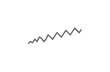
\begin{tikzpicture}[x=0.08em, y=0.08em, line width=0.4pt]
                \draw[FooterGray] (0,3) -- (1,4) -- (2,3.5) -- (3,5) -- (4,4) -- (5,6) -- (6,5.5) -- (7,4) -- (8,5) -- (9,7) -- (10,6) -- (11,5) -- (12,6.5) -- (13,8) -- (14,7) -- (15,6) -- (16,7.5) -- (17,9) -- (18,8) -- (19,7) -- (20,8.5) -- (21,10) -- (22,9) -- (23,8) -- (24,9.5);
            \end{tikzpicture}%
        }%
        \hskip0.5cm%
    }%
    \vskip6pt%
}

%=============================================================================
% PACKAGES
%=============================================================================
\usepackage[utf8]{inputenc}
\usepackage[T1]{fontenc}
\usepackage{amsmath, amssymb, amsthm}
\usepackage{mathtools}
\usepackage{bm}
\usepackage{tikz}
\usetikzlibrary{arrows.meta, positioning, shapes, calc, decorations.pathreplacing, shadings}
\usepackage{booktabs}
\usepackage{multirow}
\usepackage{array}
\usepackage{graphicx}
\usepackage{hyperref}
\usepackage{colortbl}
\hypersetup{colorlinks=true, linkcolor=MainBlue, urlcolor=MainBlue}
\graphicspath{{../logos/}{../charts/}}

%=============================================================================
% QUANTLET COMMAND
%=============================================================================
\newcommand{\quantlet}[2]{%
    \hfill\href{#2}{%
        \raisebox{-0.15em}{\includegraphics[height=0.7em]{ql_logo.png}}%
        \textcolor{MainBlue}{\tiny\ #1}%
    }%
}

%=============================================================================
% CUSTOM TITLE PAGE
%=============================================================================
\defbeamertemplate*{title page}{hybrid}[1][]
{
    \vspace{0.2cm}
    % Logos row - top header (with clickable links)
    \begin{center}
        \href{https://www.ase.ro}{\includegraphics[height=0.95cm]{ase_logo.png}}\hspace{0.25cm}%
        \href{https://theida.net}{\includegraphics[height=0.95cm]{ida_logo.png}}\hspace{0.25cm}%
        \href{https://blockchain-research-center.com}{\includegraphics[height=0.95cm]{brc_logo.png}}\hspace{0.25cm}%
        \href{https://www.ai4efin.ase.ro}{\includegraphics[height=0.95cm]{ai4efin_logo.png}}\hspace{0.25cm}%
        \href{https://ipe.ro/new}{\includegraphics[height=0.95cm]{acad_logo.png}}\hspace{0.25cm}%
        \href{https://www.digital-finance-msca.com}{\includegraphics[height=0.95cm]{msca_logo.png}}%
    \end{center}

    \vspace{0.6cm}

    % Main title with Q logos on sides (with clickable links)
    \begin{center}
        \makebox[\textwidth][c]{%
        \begin{minipage}{0.08\textwidth}
            \centering
            \href{https://quantlet.com}{\includegraphics[height=0.9cm]{ql_logo.png}}
        \end{minipage}%
        \begin{minipage}{0.76\textwidth}
            \centering
            {\LARGE\bfseries\usebeamercolor[fg]{title}\inserttitle}

            \vspace{0.25cm}

            {\usebeamerfont{subtitle}\usebeamercolor[fg]{title}\insertsubtitle}
        \end{minipage}%
        \begin{minipage}{0.08\textwidth}
            \centering
            \href{https://quantinar.com}{\includegraphics[height=0.9cm]{qr_logo.png}}
        \end{minipage}%
        }
    \end{center}

    \vspace{0.6cm}

    % Authors (left aligned)
    \hspace{0.5cm}{\usebeamerfont{author}\insertauthor}

    \vspace{0.3cm}

    % Institute/Affiliations (left aligned)
    \hspace{0.5cm}\begin{minipage}[t]{0.85\textwidth}
        \raggedright\small\insertinstitute
    \end{minipage}
}

%=============================================================================
% THEOREM ENVIRONMENTS
%=============================================================================
\theoremstyle{definition}
\setbeamertemplate{theorems}[numbered]
\newtheorem{defn}{Definition}
\newtheorem{thm}{Theorem}
\newtheorem{prop}{Proposition}
\newtheorem{rmk}{Remark}

%=============================================================================
% CUSTOM COMMANDS
%=============================================================================
\newcommand{\E}{\mathbb{E}}
\newcommand{\Var}{\text{Var}}
\newcommand{\Cov}{\text{Cov}}
\newcommand{\Corr}{\text{Corr}}
\newcommand{\R}{\mathbb{R}}
\newcommand{\N}{\mathbb{N}}
\newcommand{\Z}{\mathbb{Z}}
\newcommand{\RMSE}{\text{RMSE}}
\newcommand{\MAE}{\text{MAE}}
\newcommand{\MAPE}{\text{MAPE}}

%=============================================================================
% TITLE INFORMATION
%=============================================================================
\title[Time Series Analysis]{Time Series Analysis and Forecasting}
\subtitle{Chapter 1: Stochastic Processes and Stationarity}
\author[D.T. Pele]{Daniel Traian PELE}
\institute{Bucharest University of Economic Studies\\
IDA Institute Digital Assets\\
Blockchain Research Center\\
AI4EFin Artificial Intelligence for Energy Finance\\
Romanian Academy, Institute for Economic Forecasting\\
MSCA Digital Finance}
\date{}

\begin{document}

% Title page (no header/footer)
{
\setbeamertemplate{headline}{}
\setbeamertemplate{footline}{}
\begin{frame}
    \titlepage
\end{frame}
}

%=============================================================================
% COURSE OBJECTIVES
%=============================================================================
\begin{frame}{Learning Objectives}
    \textbf{\large By the end of this chapter, you will be able to:}
    \vspace{0.15cm}
    \begin{enumerate}
        \item[\textcolor{MainBlue}{\textbf{1.}}] \textbf{Define} stochastic processes and understand their properties
        \vspace{0.08cm}
        \item[\textcolor{MainBlue}{\textbf{2.}}] \textbf{Distinguish} between strict and weak (covariance) stationarity
        \vspace{0.08cm}
        \item[\textcolor{MainBlue}{\textbf{3.}}] \textbf{Identify} white noise and random walk processes
        \vspace{0.08cm}
        \item[\textcolor{MainBlue}{\textbf{4.}}] \textbf{Compute} and interpret ACF and PACF
        \vspace{0.08cm}
        \item[\textcolor{MainBlue}{\textbf{5.}}] \textbf{Apply} the lag operator and differencing
        \vspace{0.08cm}
        \item[\textcolor{MainBlue}{\textbf{6.}}] \textbf{Conduct} stationarity tests (ADF, KPSS)
        \vspace{0.08cm}
        \item[\textcolor{MainBlue}{\textbf{7.}}] \textbf{Analyze} financial time series data
        \vspace{0.08cm}
        \item[\textcolor{MainBlue}{\textbf{8.}}] \textbf{Distinguish} between unit root and trend-stationary processes
    \end{enumerate}
\end{frame}

%=============================================================================
% TABLE OF CONTENTS
%=============================================================================
\begin{frame}{Chapter Outline}
    \setbeamertemplate{section in toc}{\color{MainBlue}$\boxdot$~\inserttocsection}
    \tableofcontents
\end{frame}

%=============================================================================
% SECTION: MOTIVATION
%=============================================================================
\section{Motivation}

\begin{frame}{Why Study Time Series?}
    \begin{center}
        \includegraphics[width=0.95\textwidth, height=0.55\textheight, keepaspectratio]{ch1_motivation_everywhere.pdf}
    \end{center}
    \vspace{-0.2cm}
    \begin{exampleblock}{Time Series Are Everywhere}
        Finance (stock prices), Economics (GDP, inflation), Climate (temperature), Healthcare (patient monitoring), Energy (demand forecasting), and more.
    \end{exampleblock}
\end{frame}

\begin{frame}{Time Series Components}
    \begin{center}
        \includegraphics[width=0.95\textwidth, height=0.55\textheight, keepaspectratio]{ch1_motivation_components.pdf}
    \end{center}
    \vspace{-0.2cm}
    \begin{block}{Understanding Structure}
        Real time series often contain: \textbf{Trend} (long-term direction), \textbf{Seasonality} (repeating patterns), and \textbf{Irregular} (random fluctuations).
    \end{block}
\end{frame}

\begin{frame}{The Ultimate Goal: Forecasting}
    \begin{center}
        \includegraphics[width=0.95\textwidth, height=0.55\textheight, keepaspectratio]{ch1_motivation_forecast.pdf}
    \end{center}
    \vspace{-0.2cm}
    \begin{alertblock}{Why Forecasting Matters}
        Accurate predictions enable better decisions: inventory management, financial planning, risk assessment, and resource allocation.
    \end{alertblock}
\end{frame}

%=============================================================================
% SECTION 1: STOCHASTIC PROCESSES
%=============================================================================
\section{Stochastic Processes}

\begin{frame}{Stochastic Process: Definition}
    \begin{defn}[Stochastic Process]
        A \textbf{stochastic process} is a collection of random variables indexed by time:
        \[
            \{X_t(\omega) : t \in \mathcal{T}, \omega \in \Omega\}
        \]
        where $\Omega$ is the sample space of possible outcomes.
    \end{defn}

    \vspace{0.1cm}

    \begin{columns}[T]
        \column{0.48\textwidth}
        \begin{block}{Two Perspectives}
            \begin{itemize}
                \item \textbf{Fixed $\omega$}: A \textit{realization} $\{X_t(\omega)\}_{t \in \mathcal{T}}$
                \item \textbf{Fixed $t$}: A \textit{random variable} $X_t$
            \end{itemize}
        \end{block}
        \column{0.5\textwidth}
        \begin{exampleblock}{Key Insight}
            A time series we observe is \textbf{one realization} of the underlying stochastic process.
        \end{exampleblock}
    \end{columns}
\end{frame}

\begin{frame}{Stochastic Process: Visual Illustration}
    \begin{center}
        \includegraphics[width=0.95\textwidth, height=0.65\textheight, keepaspectratio]{ch1_def_stochastic.pdf}
    \end{center}
    \vspace{-0.2cm}
    \begin{exampleblock}{Interpretation}
        \small Each line is a different realization from the same stochastic process. We observe only one realization but want to understand the process.
    \end{exampleblock}
\end{frame}

\begin{frame}{Moments of a Stochastic Process}
    \begin{block}{First Two Moments Characterize Weak Properties}
        \textbf{Mean Function:} \quad $\mu_t = \E[X_t]$

        \vspace{0.1cm}

        \textbf{Autocovariance Function (ACVF):}
        \[
            \gamma(t, s) = \Cov(X_t, X_s) = \E[(X_t - \mu_t)(X_s - \mu_s)]
        \]

        \textbf{Autocorrelation Function (ACF):}
        \[
            \rho(t, s) = \frac{\gamma(t, s)}{\sqrt{\Var(X_t) \cdot \Var(X_s)}}
        \]
    \end{block}

    \begin{columns}[T]
        \column{0.5\textwidth}
        \begin{exampleblock}{Properties}
            $\rho(t, s) \in [-1, 1]$ and $\rho(t, t) = 1$
        \end{exampleblock}
        \column{0.48\textwidth}
        \begin{alertblock}{Key Point}
            In general, $\mu_t$ and $\gamma(t,s)$ may depend on $t$.
        \end{alertblock}
    \end{columns}
\end{frame}

%=============================================================================
% SECTION 4: STATIONARITY
%=============================================================================
\section{Stationarity}

\begin{frame}{Why Stationarity Matters}
    \textbf{Stationarity} is a fundamental assumption for time series analysis:

    \vspace{0.15cm}

    \begin{columns}[T]
        \begin{column}{0.48\textwidth}
            \textbf{\textcolor{Crimson}{Without Stationarity:}}
            \begin{itemize}
                \item Mean, variance change over time
                \item Past may not predict future
                \item Standard methods fail
                \item Spurious correlations
            \end{itemize}
        \end{column}
        \begin{column}{0.48\textwidth}
            \textbf{\textcolor{Forest}{With Stationarity:}}
            \begin{itemize}
                \item Statistical properties constant
                \item Can estimate from one realization
                \item Valid inference possible
                \item Models are meaningful
            \end{itemize}
        \end{column}
    \end{columns}

    \vspace{0.2cm}

    \begin{alertblock}{Key Principle}
        Most time series models (ARMA, ARIMA, etc.) require stationarity. Non-stationary series must be transformed (e.g., differencing) before modeling.
    \end{alertblock}
\end{frame}

\begin{frame}{Stationary vs Non-Stationary: Visual Comparison}
    \vspace{-0.3cm}
    \begin{center}
        \includegraphics[width=0.95\textwidth, height=0.62\textheight, keepaspectratio]{ch1_stationarity.pdf}
    \end{center}
    \vspace{-0.2cm}
    {\footnotesize
    \begin{itemize}
        \item \textbf{Stationary}: Constant mean and variance -- fluctuates around a fixed level
        \item \textbf{Non-stationary}: Mean and/or variance change over time
        \item Visual inspection is the first step; formal tests (ADF, KPSS) confirm
    \end{itemize}
    }\quantlet{TSA\_ch1\_stationarity}{https://github.com/QuantLet/TSA/tree/main/ch1_stationarity}
\end{frame}

\begin{frame}{Strict Stationarity}
    \begin{defn}[Strict (Strong) Stationarity]
        A process $\{X_t\}$ is \textbf{strictly stationary} if for all $k$, all $t_1, \ldots, t_k$, and all $h$:
        \[
            (X_{t_1}, X_{t_2}, \ldots, X_{t_k}) \stackrel{d}{=} (X_{t_1+h}, X_{t_2+h}, \ldots, X_{t_k+h})
        \]
    \end{defn}

    \begin{columns}[T]
        \column{0.55\textwidth}
        \begin{block}{Implications}
            \begin{itemize}
                \item All marginal distributions $F_{X_t}(x)$ identical
                \item $\E[X_t] = \mu$ (constant mean)
                \item $\Var(X_t) = \sigma^2$ (constant variance)
                \item Joint distributions depend only on lag
            \end{itemize}
        \end{block}
        \column{0.43\textwidth}
        \begin{alertblock}{Note}
            Strict stationarity is a strong condition, often impractical to verify.
        \end{alertblock}
    \end{columns}
\end{frame}

\begin{frame}{Strict Stationarity: Visual Illustration}
    \begin{center}
        \includegraphics[width=0.95\textwidth, height=0.65\textheight, keepaspectratio]{ch1_def_strict_stationarity.pdf}
    \end{center}
    \vspace{-0.2cm}
    \begin{exampleblock}{Interpretation}
        \small Stationary: any two windows have the same joint distribution. Non-stationary: distribution changes over time.
    \end{exampleblock}
\end{frame}

\begin{frame}{Weak (Covariance) Stationarity}
    \begin{defn}[Weak Stationarity]
        A process $\{X_t\}$ is \textbf{weakly stationary} (or covariance stationary) if:
        \begin{enumerate}
            \item $\E[X_t] = \mu$ \quad (constant mean)
            \item $\Var(X_t) = \sigma^2 < \infty$ \quad (constant, finite variance)
            \item $\Cov(X_t, X_{t+h}) = \gamma(h)$ \quad (covariance depends only on lag $h$)
        \end{enumerate}
    \end{defn}

    \vspace{0.15cm}

    \textbf{Key property:} Autocovariance is a function of lag only:
    \begin{equation}
        \gamma(h) = \Cov(X_t, X_{t+h}) = \E[(X_t - \mu)(X_{t+h} - \mu)]
    \end{equation}

    \textbf{Autocorrelation function:}
    \begin{equation}
        \rho(h) = \frac{\gamma(h)}{\gamma(0)} = \frac{\Cov(X_t, X_{t+h})}{\Var(X_t)}
    \end{equation}

    Note: $\rho(0) = 1$ and $\rho(h) = \rho(-h)$ (symmetry)
\end{frame}

\begin{frame}{Weak Stationarity: Visual Illustration}
    \begin{center}
        \includegraphics[width=0.95\textwidth, height=0.65\textheight, keepaspectratio]{ch1_def_weak_stationarity.pdf}
    \end{center}
    \vspace{-0.2cm}
    \begin{exampleblock}{Interpretation}
        \small Left: constant mean and variance. Right: autocovariance depends only on lag $h$, not time $t$.
    \end{exampleblock}
\end{frame}

\begin{frame}{Properties of the Autocovariance Function}
    \begin{block}{ACVF Properties for Weakly Stationary Process}
        The ACVF $\gamma(h)$ satisfies:
        \begin{enumerate}
            \item \textbf{Symmetry:} $\gamma(h) = \gamma(-h)$
            \item \textbf{Maximum at zero:} $|\gamma(h)| \leq \gamma(0)$
            \item \textbf{Non-negative definiteness}
        \end{enumerate}
    \end{block}

    \vspace{0.2cm}

    \begin{alertblock}{Implication}
        Not every function can be an autocovariance function.
    \end{alertblock}
\end{frame}

%=============================================================================
% SECTION 5: WHITE NOISE AND RANDOM WALK
%=============================================================================
\section{White Noise and Random Walk}

\begin{frame}{White Noise Process}
    \begin{defn}[White Noise]
        A process $\{\varepsilon_t\}$ is \textbf{white noise}, denoted $\varepsilon_t \sim WN(0, \sigma^2)$, if:
        \begin{enumerate}
            \item $\E[\varepsilon_t] = 0$ for all $t$
            \item $\Var(\varepsilon_t) = \sigma^2$ for all $t$
            \item $\Cov(\varepsilon_t, \varepsilon_s) = 0$ for $t \neq s$
        \end{enumerate}
    \end{defn}

    \begin{columns}[T]
        \column{0.45\textwidth}
        \begin{block}{ACF of White Noise}
            \[
                \rho(h) = \begin{cases}
                    1 & \text{if } h = 0 \\
                    0 & \text{if } h \neq 0
                \end{cases}
            \]
        \end{block}
        \column{0.53\textwidth}
        \begin{exampleblock}{Types}
            \begin{itemize}
                \item \textbf{Weak}: Uncorrelated
                \item \textbf{Strong}: i.i.d.
                \item \textbf{Gaussian}: $\varepsilon_t \stackrel{iid}{\sim} N(0, \sigma^2)$
            \end{itemize}
        \end{exampleblock}
    \end{columns}
\end{frame}

\begin{frame}{White Noise vs Random Walk: Comparison}
    \vspace{-0.3cm}
    \begin{center}
        \includegraphics[width=0.95\textwidth, height=0.62\textheight, keepaspectratio]{ch1_wn_rw.pdf}
    \end{center}
    \vspace{-0.2cm}
    {\footnotesize
    \begin{itemize}
        \item \textbf{White noise}: Fluctuates around zero -- stationary, constant variance
        \item \textbf{Random walk}: Cumulative sum of white noise -- wanders away, non-stationary
        \item Random walk is the simplest non-stationary process (unit root)
    \end{itemize}
    }\quantlet{TSA\_ch1\_wn\_rw}{https://github.com/QuantLet/TSA/tree/main/ch1_wn_rw}
\end{frame}

\begin{frame}{White Noise: Visual Illustration}
    \begin{center}
        \includegraphics[width=0.95\textwidth, height=0.65\textheight, keepaspectratio]{ch1_def_white_noise.pdf}
    \end{center}
    \vspace{-0.2cm}
    \begin{exampleblock}{Interpretation}
        \small Left: white noise fluctuates around zero with constant variance. Right: ACF shows no autocorrelation (all zero after lag 0).
    \end{exampleblock}
\end{frame}

\begin{frame}{Random Walk Process}
    \begin{block}{Definition}
        $X_t = X_{t-1} + \varepsilon_t$ where $\varepsilon_t \sim WN(0, \sigma^2)$, $X_0 = 0$

        \textbf{Explicit form:} $X_t = \sum_{i=1}^{t} \varepsilon_i$
    \end{block}

    \begin{columns}[T]
        \column{0.5\textwidth}
        \begin{exampleblock}{Properties}
            \begin{itemize}
                \item $\E[X_t] = 0$ (constant mean)
                \item $\Var(X_t) = t\sigma^2$ (grows with time!)
                \item $\Cov(X_t, X_s) = \min(t, s) \cdot \sigma^2$
            \end{itemize}
        \end{exampleblock}
        \column{0.48\textwidth}
        \begin{alertblock}{Non-Stationary!}
            Random walk is \textbf{not stationary} because variance depends on $t$.
        \end{alertblock}
    \end{columns}
\end{frame}

\begin{frame}{Random Walk: Visualization}
    \begin{center}
        \includegraphics[width=0.95\textwidth, height=0.65\textheight, keepaspectratio]{random_walk.pdf}
    \end{center}
    \vspace{-0.2cm}
    \begin{exampleblock}{Interpretation}
        \small \textbf{Left:} Multiple paths diverge over time. \textbf{Right:} Variance grows linearly: $\Var(X_t) = t\sigma^2$.
    \end{exampleblock}
\end{frame}

\begin{frame}{ACF Comparison: Stationary vs Random Walk}
    \begin{center}
        \includegraphics[width=0.95\textwidth, height=0.65\textheight, keepaspectratio]{rw_vs_stationary.pdf}
    \end{center}
    \vspace{-0.2cm}
    \begin{exampleblock}{Key Diagnostic}
        \small ACF of stationary process decays quickly; ACF of random walk decays very slowly.
    \end{exampleblock}
\end{frame}

%=============================================================================
% SECTION 6: ACF AND PACF
%=============================================================================
\section{Autocorrelation Functions}

\begin{frame}{Sample Autocorrelation Function}
    \begin{block}{Sample ACF at Lag $h$}
        \begin{equation}
            \hat{\rho}(h) = \frac{\sum_{t=1}^{T-h}(x_t - \bar{x})(x_{t+h} - \bar{x})}{\sum_{t=1}^{T}(x_t - \bar{x})^2}
        \end{equation}
    \end{block}

    \begin{columns}[T]
        \column{0.45\textwidth}
        \begin{exampleblock}{Properties}
            \begin{itemize}
                \item $\hat{\rho}(0) = 1$ always
                \item $|\hat{\rho}(h)| \leq 1$
            \end{itemize}
        \end{exampleblock}
        \column{0.53\textwidth}
        \begin{alertblock}{Significance Test}
            Under white noise: $\hat{\rho}(h) \approx N(0, 1/T)$

            \textbf{95\% bounds:} $\pm 1.96/\sqrt{T}$
        \end{alertblock}
    \end{columns}
\end{frame}

\begin{frame}{ACF Patterns for Different Processes}
    \vspace{-0.3cm}
    \begin{center}
        \includegraphics[width=0.95\textwidth, height=0.62\textheight, keepaspectratio]{ch1_acf_examples.pdf}
    \end{center}
    \vspace{-0.2cm}
    {\footnotesize
    \begin{itemize}
        \item \textbf{White noise}: ACF drops to zero immediately (no dependence)
        \item \textbf{AR(1)}: ACF decays exponentially -- indicates autoregressive structure
        \item \textbf{Seasonal}: ACF shows spikes at seasonal lags (e.g., 12, 24 for monthly)
        \item \textbf{Random walk}: ACF decays very slowly -- sign of non-stationarity
    \end{itemize}
    }\quantlet{TSA\_ch1\_acf\_examples}{https://github.com/QuantLet/TSA/tree/main/ch1_acf_examples}
\end{frame}

\begin{frame}{Partial Autocorrelation Function (PACF)}
    \begin{block}{Definition}
        \textbf{PACF} $\phi_{hh}$: Correlation between $X_t$ and $X_{t+h}$ after removing the linear effect of $X_{t+1}, \ldots, X_{t+h-1}$.
    \end{block}

    \begin{columns}[T]
        \column{0.48\textwidth}
        \begin{exampleblock}{Interpretation}
            \begin{itemize}
                \item $\phi_{11} = \rho(1)$ (same as ACF at lag 1)
                \item $\phi_{22}$: correlation controlling for $X_{t+1}$
                \item Measures \textit{direct} dependence
            \end{itemize}
        \end{exampleblock}
        \column{0.5\textwidth}
        \begin{alertblock}{Key Application}
            \begin{itemize}
                \item AR($p$): PACF \textbf{cuts off} after lag $p$
                \item MA($q$): ACF \textbf{cuts off} after lag $q$
            \end{itemize}
        \end{alertblock}
    \end{columns}
\end{frame}

\begin{frame}{ACF and PACF Patterns}
    \begin{center}
        \includegraphics[width=0.95\textwidth, height=0.82\textheight, keepaspectratio]{acf_pacf_examples.pdf}
    \end{center}
\end{frame}

\begin{frame}{Theoretical ACF for AR(1)}
    \begin{center}
        \includegraphics[width=0.95\textwidth, height=0.68\textheight, keepaspectratio]{acf_theoretical.pdf}
    \end{center}
    \vspace{-0.2cm}
    \begin{exampleblock}{Interpretation}
        \small For AR(1): $X_t = \phi X_{t-1} + \varepsilon_t$, the theoretical ACF is $\rho(h) = \phi^h$.
    \end{exampleblock}
\end{frame}

%=============================================================================
% SECTION 7: LAG OPERATOR AND DIFFERENCING
%=============================================================================
\section{Lag Operator and Differencing}

\begin{frame}{The Lag Operator}
    \begin{defn}[Lag Operator]
        The \textbf{lag operator} (or backshift operator) $L$ is defined by:
        \[
            LX_t = X_{t-1}
        \]
    \end{defn}

    \begin{columns}[T]
        \column{0.48\textwidth}
        \begin{block}{Properties}
            \begin{itemize}
                \item $L^k X_t = X_{t-k}$ (lag by $k$ periods)
                \item $L^0 = I$ (identity)
                \item $(1 - \phi L)X_t = X_t - \phi X_{t-1}$
            \end{itemize}
        \end{block}
        \column{0.5\textwidth}
        \begin{exampleblock}{Examples}
            \begin{itemize}
                \item AR(1): $(1 - \phi L)X_t = \varepsilon_t$
                \item MA(1): $X_t = (1 + \theta L)\varepsilon_t$
                \item AR($p$): $\phi(L)X_t = \varepsilon_t$
            \end{itemize}
        \end{exampleblock}
    \end{columns}
\end{frame}

\begin{frame}{Lag Operator: Visual Illustration}
    \begin{center}
        \includegraphics[width=0.95\textwidth, height=0.65\textheight, keepaspectratio]{ch1_def_lag_operator.pdf}
    \end{center}
    \vspace{-0.2cm}
    \begin{exampleblock}{Interpretation}
        \small The lag operator $L$ shifts every observation back by one time period: $LX_t = X_{t-1}$.
    \end{exampleblock}
\end{frame}

\begin{frame}{Differencing}
    \begin{block}{First Difference}
        $\Delta X_t = X_t - X_{t-1} = (1 - L)X_t$
    \end{block}

    \begin{columns}[T]
        \column{0.48\textwidth}
        \begin{exampleblock}{Why Difference?}
            \begin{itemize}
                \item Removes trend and unit root
                \item Random walk: $\Delta X_t = \varepsilon_t$ (white noise)
            \end{itemize}
        \end{exampleblock}
        \column{0.5\textwidth}
        \begin{block}{Integrated Process}
            $X_t \sim I(d)$ if $\Delta^d X_t$ is stationary
            \begin{itemize}
                \item $I(0)$: Stationary (no differencing)
                \item $I(1)$: One difference needed
                \item $I(2)$: Two differences needed
            \end{itemize}
        \end{block}
    \end{columns}
\end{frame}

\begin{frame}{Effect of Differencing: S\&P 500}
    \begin{center}
        \includegraphics[width=0.95\textwidth, height=0.82\textheight, keepaspectratio]{differencing_effect.pdf}
    \end{center}
\end{frame}

%=============================================================================
% SECTION 8: TESTING FOR STATIONARITY
%=============================================================================
\section{Testing for Stationarity}

\begin{frame}{Augmented Dickey-Fuller (ADF) Test}
    \begin{block}{Model}
        $\Delta X_t = \alpha + \gamma X_{t-1} + \sum_{i=1}^{p} \delta_i \Delta X_{t-i} + \varepsilon_t$
    \end{block}

    \vspace{0.1cm}

    \begin{columns}[T]
        \begin{column}{0.48\textwidth}
            \begin{exampleblock}{Hypotheses}
                \begin{itemize}
                    \item $H_0$: $\gamma = 0$ (unit root)
                    \item $H_1$: $\gamma < 0$ (stationary)
                \end{itemize}
            \end{exampleblock}
        \end{column}
        \begin{column}{0.48\textwidth}
            \begin{block}{Test Statistic}
                \[
                    \tau = \frac{\hat{\gamma}}{SE(\hat{\gamma})}
                \]
            \end{block}
        \end{column}
    \end{columns}

    \vspace{0.1cm}

    \begin{alertblock}{Decision Rule}
        $\tau <$ critical value $\Rightarrow$ Reject $H_0$ $\Rightarrow$ \textcolor{Forest}{Stationary} \\
        $\tau \geq$ critical value $\Rightarrow$ \textcolor{Crimson}{Non-stationary}
    \end{alertblock}
\end{frame}

\begin{frame}{KPSS Test}
    \begin{block}{Model}
        $X_t = \xi t + r_t + \varepsilon_t$ where $r_t = r_{t-1} + u_t$
    \end{block}

    \vspace{0.1cm}

    \begin{columns}[T]
        \begin{column}{0.48\textwidth}
            \begin{exampleblock}{Hypotheses (opposite of ADF)}
                \begin{itemize}
                    \item $H_0$: $\sigma_u^2 = 0$ (stationary)
                    \item $H_1$: $\sigma_u^2 > 0$ (unit root)
                \end{itemize}
            \end{exampleblock}
        \end{column}
        \begin{column}{0.48\textwidth}
            \begin{block}{Test Statistic}
                \[
                    LM = \frac{\sum_{t=1}^{T} S_t^2}{T^2 \hat{\sigma}^2}
                \]
                {\small where $S_t = \sum_{i=1}^{t} \hat{e}_i$}
            \end{block}
        \end{column}
    \end{columns}

    \vspace{0.1cm}

    \begin{alertblock}{Decision Rule}
        $LM >$ critical value $\Rightarrow$ Reject $H_0$ $\Rightarrow$ \textcolor{Crimson}{Non-stationary} \\
        $LM \leq$ critical value $\Rightarrow$ \textcolor{Forest}{Stationary}
    \end{alertblock}
\end{frame}

\begin{frame}{Using ADF and KPSS Together}
    \begin{block}{Confirmatory Testing for Robust Conclusions}
        \begin{center}
        \small
        \begin{tabular}{lccl}
            \toprule
            \textbf{ADF} & \textbf{KPSS} & \textbf{Conclusion} \\
            \midrule
            Reject $H_0$ & Fail to reject $H_0$ & \textcolor{Forest}{Stationary} \\
            Fail to reject $H_0$ & Reject $H_0$ & \textcolor{Crimson}{Unit Root} \\
            Reject $H_0$ & Reject $H_0$ & Inconclusive \\
            Fail to reject $H_0$ & Fail to reject $H_0$ & Inconclusive \\
            \bottomrule
        \end{tabular}
        \end{center}
    \end{block}

    \begin{exampleblock}{Recommended Workflow}
        \begin{enumerate}
            \item Run ADF test (null = unit root)
            \item Run KPSS test (null = stationary)
            \item If results agree, proceed with confidence
            \item If inconclusive, consider alternative tests (PP, DF-GLS)
        \end{enumerate}
    \end{exampleblock}
\end{frame}

\begin{frame}{ADF Test: Visualization with S\&P 500}
    \begin{center}
        \includegraphics[width=0.95\textwidth, height=0.82\textheight, keepaspectratio]{adf_test_visualization.pdf}
    \end{center}
\end{frame}

%=============================================================================
% SECTION 9: REAL DATA APPLICATION
%=============================================================================
\section{Financial Data Application}

\begin{frame}{S\&P 500 Analysis: Overview}
    \begin{center}
        \includegraphics[width=0.95\textwidth, height=0.82\textheight, keepaspectratio]{sp500_analysis.pdf}
    \end{center}
\end{frame}

\begin{frame}{Stylized Facts of Financial Returns}
    \begin{center}
        \includegraphics[width=0.95\textwidth, height=0.48\textheight, keepaspectratio]{returns_distribution.pdf}
    \end{center}
    \vspace{-0.1cm}
    \begin{columns}[T]
        \begin{column}{0.48\textwidth}
            \textbf{Observed properties:}
            \begin{itemize}
                \item Negative skewness (left tail)
                \item Excess kurtosis ($\gg 3$)
                \item Heavy tails (fat tails)
            \end{itemize}
        \end{column}
        \begin{column}{0.48\textwidth}
            \textbf{Implications:}
            \begin{itemize}
                \item Normal distribution inadequate
                \item Extreme events more likely
                \item Need Student-t or similar
            \end{itemize}
        \end{column}
    \end{columns}
\end{frame}

\begin{frame}{Volatility Clustering}
    \begin{center}
        \includegraphics[width=0.95\textwidth, height=0.55\textheight, keepaspectratio]{volatility_clustering.pdf}
    \end{center}
    \vspace{-0.1cm}
    \begin{alertblock}{Stylized Fact}
        Large returns (positive or negative) tend to be followed by large returns. This \textbf{volatility clustering} motivates ARCH/GARCH models (future chapters).
    \end{alertblock}
\end{frame}

%=============================================================================
% SECTION 10: SUMMARY
%=============================================================================
\section{Summary}

\begin{frame}{Key Takeaways}
    \begin{block}{Summary}
    \small
    \begin{enumerate}
        \item \textbf{Time series} = observations indexed by time with temporal dependence
        \item \textbf{Decomposition}: Additive $X_t = T_t + S_t + \varepsilon_t$ or Multiplicative
        \item \textbf{Exponential Smoothing}: SES (level), Holt (trend), Holt-Winters (seasonal)
        \item \textbf{Forecast Evaluation}: MAE, RMSE, MAPE; use train/validation/test splits
        \item \textbf{Seasonality Modeling}: Dummy variables (any pattern) or Fourier terms (smooth)
        \item \textbf{Trend Handling}: Differencing (stochastic) or regression (deterministic)
        \item \textbf{Stationarity}: Mean, variance, autocovariance constant over time
        \item \textbf{ACF/PACF}: Essential for identifying dependence structure
        \item \textbf{Unit root tests}: ADF ($H_0$: unit root) vs KPSS ($H_0$: stationary)
    \end{enumerate}
    \end{block}
\end{frame}

\begin{frame}{Important Formulas I}
    \begin{block}{Decomposition}
        Additive: $X_t = T_t + S_t + \varepsilon_t$ \quad Multiplicative: $X_t = T_t \times S_t \times \varepsilon_t$
    \end{block}

    \begin{block}{Simple Exponential Smoothing (SES)}
        $\hat{X}_{t+1|t} = \alpha X_t + (1-\alpha)\hat{X}_{t|t-1}$ \quad where $\alpha \in (0,1)$
    \end{block}

    \begin{block}{Holt's Linear Trend}
        $\ell_t = \alpha X_t + (1-\alpha)(\ell_{t-1} + b_{t-1})$ \quad $b_t = \beta^*(\ell_t - \ell_{t-1}) + (1-\beta^*)b_{t-1}$
    \end{block}

    \begin{block}{Holt-Winters Additive}
        $\ell_t = \alpha(X_t - S_{t-s}) + (1-\alpha)(\ell_{t-1} + b_{t-1})$ \quad $S_t = \gamma(X_t - \ell_t) + (1-\gamma)S_{t-s}$
    \end{block}
\end{frame}

\begin{frame}{Important Formulas II}
    \begin{block}{Moving Average (Trend Estimation)}
        $\hat{T}_t = \frac{1}{2q+1}\sum_{j=-q}^{q} X_{t+j}$
    \end{block}

    \begin{block}{Autocovariance and Autocorrelation}
        $\gamma(h) = \Cov(X_t, X_{t+h})$ \qquad $\rho(h) = \frac{\gamma(h)}{\gamma(0)}$
    \end{block}

    \begin{block}{Random Walk}
        $X_t = X_{t-1} + \varepsilon_t$ \quad $\Rightarrow$ \quad $\Var(X_t) = t\sigma^2$ (non-stationary)
    \end{block}

    \begin{block}{Differencing}
        $\Delta X_t = (1-L)X_t = X_t - X_{t-1}$
    \end{block}
\end{frame}

\begin{frame}{Next Chapter Preview}
    \begin{block}{Chapter 2: ARMA Models}
        \begin{itemize}
            \item Autoregressive (AR) models
            \item Moving Average (MA) models
            \item Combined ARMA models
            \item Model identification using ACF/PACF
            \item Parameter estimation
            \item Model diagnostics
            \item Forecasting
        \end{itemize}
    \end{block}
\end{frame}

%=============================================================================
\section{Case Study: Romanian GDP}
%=============================================================================

\begin{frame}{Case Study: Romanian Quarterly GDP}
    \begin{center}
        \includegraphics[width=0.95\textwidth, height=0.70\textheight, keepaspectratio]{ch1_case_gdp_raw.pdf}
    \end{center}
    \vspace{-0.2cm}
    {\small
    \begin{itemize}
        \item \textbf{Data}: Romanian quarterly GDP, 2010--2023 (source: INS/Eurostat)
        \item \textbf{Observations}: Upward trend, quarterly seasonality, COVID-19 shock in 2020
    \end{itemize}
    }
\end{frame}

\begin{frame}{GDP Series Decomposition}
    \begin{center}
        \includegraphics[width=0.95\textwidth, height=0.78\textheight, keepaspectratio]{ch1_case_gdp_decomposition.pdf}
    \end{center}
\end{frame}

\begin{frame}{Interpreting the Components}
    \begin{columns}[T]
        \begin{column}{0.5\textwidth}
            \begin{block}{Identified Components}
                \begin{itemize}
                    \item \textbf{Trend}: Sustained economic growth
                    \item \textbf{Seasonality}: Regular quarterly pattern (Q4 > Q1)
                    \item \textbf{Residual}: Includes COVID-19 shock from 2020
                \end{itemize}
            \end{block}
        \end{column}
        \begin{column}{0.5\textwidth}
            \begin{alertblock}{Lessons Learned}
                \begin{itemize}
                    \item Decomposition helps understand data structure
                    \item External shocks (COVID) appear in residual component
                    \item Seasonality must be modeled explicitly
                \end{itemize}
            \end{alertblock}
        \end{column}
    \end{columns}

    \vspace{0.3cm}

    \begin{exampleblock}{Next Steps}
        In the following chapters we will learn to model each component: ARIMA for trend, SARIMA for seasonality.
    \end{exampleblock}
\end{frame}

%=============================================================================
% SECTION: QUIZ
%=============================================================================
\section{Quiz}

\begin{frame}{Quiz Question 1}
    \begin{alertblock}{Question}
        A time series $Y_t$ shows upward movement over years plus repeating patterns each quarter. Which components are present?
    \end{alertblock}

    \vspace{0.3cm}

    \begin{enumerate}[(A)]
        \item Trend only
        \item Seasonality only
        \item Trend and Seasonality
        \item Random noise only
    \end{enumerate}
\end{frame}

\begin{frame}{Quiz Question 1: Answer}
    \begin{center}
        \includegraphics[width=0.95\textwidth, height=0.58\textheight, keepaspectratio]{ch1_quiz1_components.pdf}
    \end{center}
    \vspace{-0.2cm}
    \begin{exampleblock}{Correct Answer: (C) Trend and Seasonality}
        Upward movement = Trend; Quarterly patterns = Seasonality (s=4)
    \end{exampleblock}
\end{frame}

\begin{frame}{Quiz Question 2}
    \begin{alertblock}{Question}
        Which of the following is a characteristic of a stationary time series?
    \end{alertblock}

    \vspace{0.3cm}

    \begin{enumerate}[(A)]
        \item Mean changes over time
        \item Variance increases with time
        \item Constant mean and variance over time
        \item Contains a trend component
    \end{enumerate}
\end{frame}

\begin{frame}{Quiz Question 2: Answer}
    \begin{center}
        \includegraphics[width=0.95\textwidth, height=0.58\textheight, keepaspectratio]{ch1_quiz2_stationarity.pdf}
    \end{center}
    \vspace{-0.2cm}
    \begin{exampleblock}{Correct Answer: (C) Constant mean and variance over time}
        Stationarity requires: constant mean, constant variance, and autocovariance depends only on lag.
    \end{exampleblock}
\end{frame}

\begin{frame}{Quiz Question 3}
    \begin{alertblock}{Question}
        For a white noise process, what does the ACF look like at lags $k > 0$?
    \end{alertblock}

    \vspace{0.3cm}

    \begin{enumerate}[(A)]
        \item Exponential decay
        \item All values significant and positive
        \item All values approximately zero (within confidence bands)
        \item Alternating positive and negative
    \end{enumerate}
\end{frame}

\begin{frame}{Quiz Question 3: Answer}
    \begin{center}
        \includegraphics[width=0.95\textwidth, height=0.58\textheight, keepaspectratio]{ch1_quiz3_acf.pdf}
    \end{center}
    \vspace{-0.2cm}
    \begin{exampleblock}{Correct Answer: (C) Approximately zero within confidence bands}
        White noise has no autocorrelation: $\rho_k = 0$ for all $k \neq 0$.
    \end{exampleblock}
\end{frame}

\begin{frame}{Quiz Question 4}
    \begin{alertblock}{Question}
        What is the key difference between white noise and a random walk?
    \end{alertblock}

    \vspace{0.3cm}

    \begin{enumerate}[(A)]
        \item White noise has a trend, random walk doesn't
        \item Random walk is the cumulative sum of white noise
        \item Both are stationary processes
        \item White noise has higher variance
    \end{enumerate}
\end{frame}

\begin{frame}{Quiz Question 4: Answer}
    \begin{center}
        \includegraphics[width=0.95\textwidth, height=0.58\textheight, keepaspectratio]{ch1_quiz4_wn_rw.pdf}
    \end{center}
    \vspace{-0.2cm}
    \begin{exampleblock}{Correct Answer: (B) Random walk = cumulative sum of white noise}
        $Y_t = Y_{t-1} + \varepsilon_t = \sum_{i=1}^t \varepsilon_i$ where $\varepsilon_t$ is white noise.
    \end{exampleblock}
\end{frame}

\begin{frame}{Quiz Question 5}
    \begin{alertblock}{Question}
        Which forecast error metric is most sensitive to large errors (outliers)?
    \end{alertblock}

    \vspace{0.3cm}

    \begin{enumerate}[(A)]
        \item MAE (Mean Absolute Error)
        \item RMSE (Root Mean Squared Error)
        \item MAPE (Mean Absolute Percentage Error)
        \item All are equally sensitive
    \end{enumerate}
\end{frame}

\begin{frame}{Quiz Question 5: Answer}
    \begin{center}
        \includegraphics[width=0.95\textwidth, height=0.58\textheight, keepaspectratio]{ch1_quiz5_forecast_errors.pdf}
    \end{center}
    \vspace{-0.2cm}
    \begin{exampleblock}{Correct Answer: (B) RMSE}
        RMSE squares errors, so large errors have disproportionate impact: $\sqrt{\frac{1}{n}\sum e_t^2}$
    \end{exampleblock}
\end{frame}

\begin{frame}{Quiz Question 6}
    \begin{alertblock}{Question}
        When should you use multiplicative decomposition instead of additive?
    \end{alertblock}

    \vspace{0.3cm}

    \begin{enumerate}[(A)]
        \item When the series has no trend
        \item When seasonal amplitude is constant
        \item When seasonal amplitude grows with the level of the series
        \item When the series is stationary
    \end{enumerate}
\end{frame}

\begin{frame}{Quiz Question 6: Answer}
    \begin{center}
        \includegraphics[width=0.95\textwidth, height=0.58\textheight, keepaspectratio]{ch1_quiz6_decomposition.pdf}
    \end{center}
    \vspace{-0.2cm}
    \begin{exampleblock}{Correct Answer: (C) Seasonal amplitude grows with level}
        Multiplicative: $Y_t = T_t \times S_t \times \varepsilon_t$ --- seasonal swings proportional to trend.
    \end{exampleblock}
\end{frame}

%=============================================================================
\section{References}
%=============================================================================

\begin{frame}{References}
    \footnotesize
    \begin{thebibliography}{99}
        \bibitem{hyndman2021} Hyndman, R.J., \& Athanasopoulos, G. (2021). \textit{Forecasting: Principles and Practice}. 3rd ed., OTexts.

        \bibitem{hamilton1994} Hamilton, J.D. (1994). \textit{Time Series Analysis}. Princeton University Press.

        \bibitem{box2015} Box, G.E.P., Jenkins, G.M., Reinsel, G.C., \& Ljung, G.M. (2015). \textit{Time Series Analysis: Forecasting and Control}. 5th ed., Wiley.

        \bibitem{tsay2010} Tsay, R.S. (2010). \textit{Analysis of Financial Time Series}. 3rd ed., Wiley.

        \bibitem{cleveland1990} Cleveland, R.B., Cleveland, W.S., McRae, J.E., \& Terpenning, I. (1990). STL: A Seasonal-Trend Decomposition. \textit{Journal of Official Statistics}, 6(1), 3-73.
    \end{thebibliography}
\end{frame}

%=============================================================================
% DATA SOURCES
%=============================================================================
\begin{frame}{Data Sources}
    \begin{block}{Real Data Used in This Chapter}
        \begin{itemize}
            \item \textbf{Airline Passengers}: Box-Jenkins classic dataset, 1949--1960
            \item \textbf{S\&P 500}: Yahoo Finance (SPY), historical data
            \item \textbf{Sunspots}: Statsmodels dataset, monthly observations
        \end{itemize}
    \end{block}

    \begin{block}{Software \& Tools}
        \begin{itemize}
            \item \textbf{Python}: statsmodels, pandas, matplotlib, yfinance
            \item \textbf{R}: forecast, tseries packages
            \item \textbf{Data Sources}: Yahoo Finance, FRED Economic Data
        \end{itemize}
    \end{block}
\end{frame}

\begin{frame}{}
    \centering
    \Huge\textcolor{MainBlue}{Thank You!}

    \vspace{1cm}

    \Large Questions?

    \vspace{0.8cm}

    \normalsize
    \textit{Charts generated using Python (statsmodels, matplotlib)}

    \vspace{0.3cm}

    Course materials available at: \url{https://github.com/danpele/Time-Series-Analysis}
\end{frame}

\end{document}
